\documentclass{article}
\usepackage[utf8]{inputenc}
\usepackage{graphicx}
\usepackage{wrapfig}
\usepackage[T1]{fontenc}
\usepackage{amssymb}
\usepackage{siunitx}

\title{Operational Amplifiers and Their Applications\\ ELP100\\Lab Report 6}
\author{Aditya Agrawal\\2021AM10198\\GROUP 29}
\date{May 31, 2022}

\begin{document}
\maketitle
\tableofcontents
\newpage

\section{Voltage Follower}
\subsection{Aim}
To setup the voltage follower and measure the output characteristics.

\subsection{Apparatus Required}
\begin{enumerate}
    \item LM741 IC
    \item Function Generator (0 – 3 MHz)
    \item Breadboard and Jumpers
    \item Multimeter and Resistors
    \item Digital Storage Oscilloscope (DSO1052B)
\end{enumerate}
\subsection{Theory}
\begin{wrapfigure}{R}{0.2\textwidth}
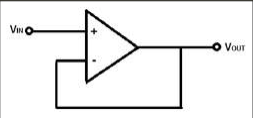
\includegraphics[width=0.3\textwidth]{i1.png}
\end{wrapfigure}
Voltage followers, also known as unity-gain amplifiers, buffer amplifiers, and isolation amplifiers, are op-amp circuits with a voltage gain of 1. This indicates that the op amp does not provide any signal amplification. Because the output voltage directly follows the input voltage, the output voltage is identical to the input voltage, hence the name voltage follower. A circuit containing an operational amplifier has a very high input impedance. Voltage followers are employed due to this high input impedance. When a circuit's input impedance is extremely high, very little current is drawn from the circuit. If you are familiar with Ohm's law, you are aware that current, I=V/R. Consequently, the greater the resistance, the lower the amount of current drawn from a power source. As a result, voltage followers consume a negligible amount of current and do not tax the power source. Since an op amp's input impedance is so high, the majority of voltage will fall across it. Therefore, its use in a voltage divider circuit is highly advantageous, as doing so strategically allows a designer to supply sufficient voltage to a load.
\begin{equation}
    V_{input}=V_{output}
\end{equation}
\newpage
\subsection{Breadboard Setup}
\begin{figure}[h!]
\centering
    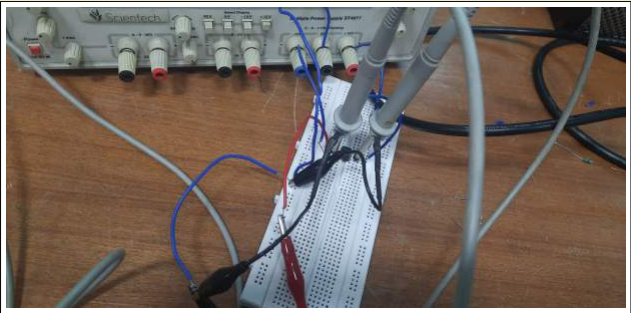
\includegraphics[width=1.1\textwidth]{i2.png}
    \caption{Circuit}
    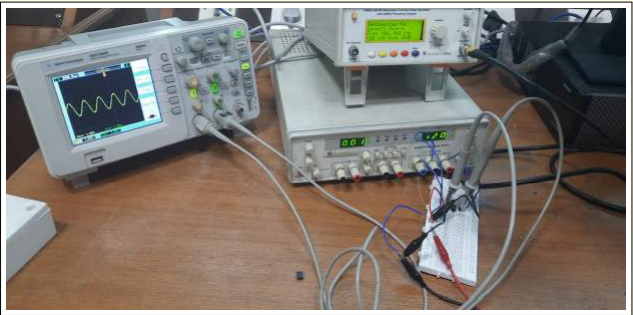
\includegraphics[width=1.1\textwidth]{i3.png}
    \caption{Circuit(with DSO)}
\end{figure}
\newpage
\subsection{DSO Images}
\begin{figure}[h]
\centering
    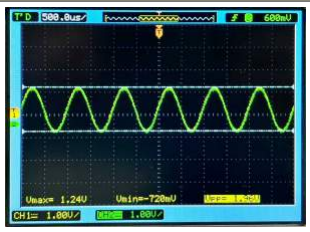
\includegraphics[width=0.5\textwidth]{i4.png}
    \caption{Voltage Follower}
    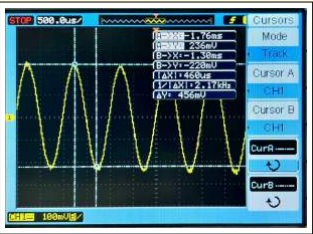
\includegraphics[width=0.5\textwidth]{i5.png}
    \caption{Voltage with 100$\Omega$ Resistor}
\end{figure}
\subsection{Observations}
\begin{center}
\begin{tabular}{|c|c|c|}
\hline
    $V_{Input}$(V) & $V_{Output}$(V) & $V_{Output}$ with Resistor(mV) \\
    \hline
    2.00 & 1.96 & 456\\
\hline
\end{tabular}
\end{center}
\subsection{Conclusion}
Thus, the Output Voltage decreases to 456mV when the 100$\Omega$ resistor is connected in parallel across the generator and the DSO input. However, when the input signal is connected to the DSO via the Voltage Follower, the op-amp maintains the input signal voltage to produce an output that is approximately the same.
\newpage
\section{Inverting Amplifier}
\subsection{Aim}
To measure the output current characteristics of an inverting amplifier.
\subsection{Apparatus Required}
\begin{enumerate}
    \item LM741 IC
    \item Function Generator (0 – 3 MHz)
    \item Breadboard and Jumpers
    \item Multimeter and Resistors
    \item Digital Storage Oscilloscope (DSO1052B)
    \item External Voltage
\end{enumerate}
\subsection{Theory}
\begin{wrapfigure}{R}{0.2\textwidth}
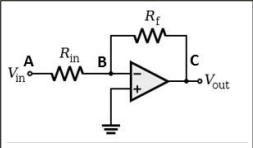
\includegraphics[width=0.55\textwidth]{i6.png}
\end{wrapfigure}
The gain equation can be derived in the following way:\\
\begin{equation}
    V_{-}\, \approx\, V_{+}\, = 0V(\textrm{Virtual Ground Method})\\
\end{equation}
By KCL:
\begin{equation}
    \frac{V_{in}}{R_{in}}\, +\, \frac{V_{out}}{R_{f}}\, =\, 0
\end{equation}
\begin{equation}
    V_{out}\, =\, -V_{in}\times \frac{R_{f}}{R_{in}}
\end{equation}
\subsection{Breadboard Setup}
\begin{figure}[h!]
\centering
    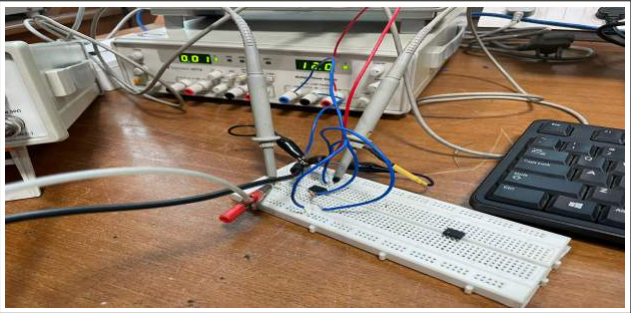
\includegraphics[width=0.6\textwidth]{i7.png}
    \caption{Circuit with $R_{in}$ = 1k$\Omega$, \textrm{and}\, $R_{f}$ = 10k$\Omega$}
\end{figure}
\subsection{DSO Images}
\begin{center}
    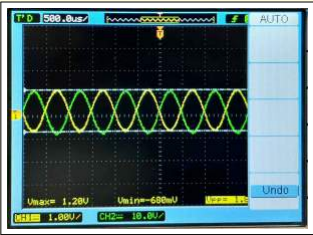
\includegraphics[width=0.4\textwidth]{i8.png}
    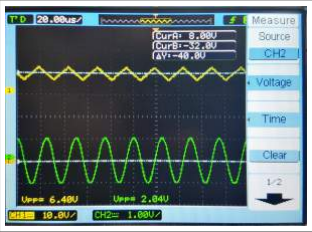
\includegraphics[width=0.4\textwidth]{i9.png}\\
    f=1kHz  $R_{f}$=10k$\Omega$ \hspace{20mm}f=40kHz  $R_{f}$=10k$\Omega$\\
    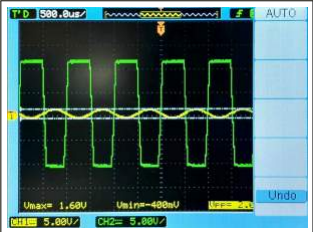
\includegraphics[width=0.4\textwidth]{i16.png}
    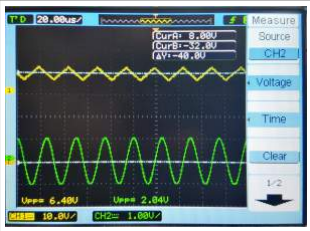
\includegraphics[width=0.4\textwidth]{i17.png}\\
    f=1kHz  $R_{f}$=47k$\Omega$\hspace{20mm}f=40kHz  $R_{f}$=47k$\Omega$\\
\end{center}
\subsection{Observations}
\begin{center}
\begin{tabular}{|c|c|c|c|}
\hline
    Frequency(kHz) & Resistance(k$\Omega$) & $Input_{PP}$(V) & $Output_{PP}$(V)\\
    \hline
    1 & 10 & 2 & -20\\
    40 & 10 & 2 & -5.4 \\
    1 & 47 & 2 & -22.4\\
    40 & 47 & 2 & -5.8\\
\hline
\end{tabular}
\end{center}
\subsection{Conclusion}
Therefore, we have determined the output signal characteristics of an op-amp in inverting configuration for a sinusoidal wave input. In accordance with the formula, the output voltage is precisely 10 times the input voltage when $R_{f}$ = 10k$\Omega$. However, the value does not exceed the supplied voltage when $R_{f}$ = 47k$\Omega$. In the shift with a higher frequency, we observe greater deviations from the expected results.
\newpage
\section{Non-Inverting Amplifier}
\subsection{Aim}
To measure the output current characteristics of an inverting amplifier.
\subsection{Apparatus Required}
\begin{enumerate}
    \item LM741 IC
    \item Function Generator (0 – 3 MHz)
    \item Breadboard and Jumpers
    \item Multimeter and Resistors
    \item Digital Storage Oscilloscope (DSO1052B)
    \item External Voltage
\end{enumerate}
\subsection{Theory}
\begin{wrapfigure}{R}{0.2\textwidth}
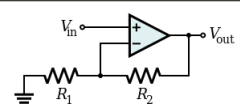
\includegraphics[width=0.5\textwidth]{i10.png}
\end{wrapfigure}
The gain equation can be derived in the following way:\\
\begin{equation}
    V_{-}\, \approx\, V_{+}\, = V_{in}(\textrm{Virtual Ground Method})\\
\end{equation}
By KCL:
\begin{equation}
    \frac{V_{in}}{R_{1}}\, +\, \frac{V_{in}-V_{out}}{R_{2}}\, =\, 0
\end{equation}
\begin{equation}
    V_{out}\, =\, V_{in}\times(1\, +\,  \frac{R_{f}}{R_{in}})
\end{equation}
\subsection{Breadboard Setup}
\begin{figure}[h!]
\centering
    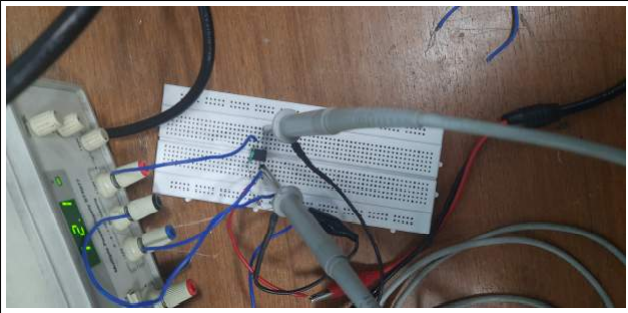
\includegraphics[width=0.6\textwidth]{i11.png}
    \caption{Circuit with $R_{1}$ = 1k$\Omega$, \textrm{and}\, $R_{2}$ = 10k$\Omega$}
\end{figure}
\subsection{DSO Images}
\begin{center}
    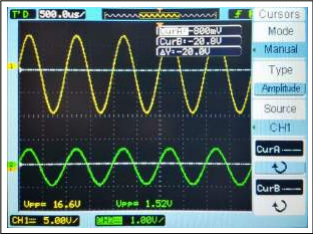
\includegraphics[width=0.4\textwidth]{i12.png}
    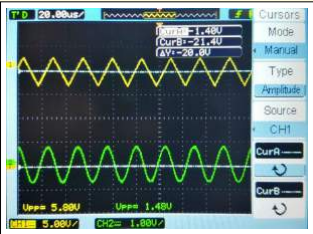
\includegraphics[width=0.4\textwidth]{i13.png}\\
    f=1kHz  $R_{f}$=10k$\Omega$ \hspace{20mm}f=40kHz  $R_{f}$=10k$\Omega$\\
    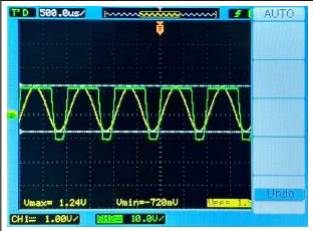
\includegraphics[width=0.4\textwidth]{i14.png}
    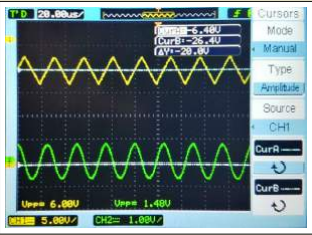
\includegraphics[width=0.4\textwidth]{i15.png}\\
    f=1kHz  $R_{f}$=47k$\Omega$\hspace{20mm}f=40kHz  $R_{f}$=47k$\Omega$\\
\end{center}
\subsection{Observations}
\begin{center}
\begin{tabular}{|c|c|c|c|}
\hline
    Frequency(kHz) & Resistance(k$\Omega$) & $Input_{PP}$(V) & $Output_{PP}$(V)\\
    \hline
    1 & 10 & 1.5 & 15.5\\
    40 & 10 & 1.5 & 5.8 \\
    1 & 47 & 1.5 & 22.4\\
    40 & 47 & 1.5 & 6.2\\
\hline
\end{tabular}
\end{center}
\subsection{Conclusion}
We observe that the phase of the current is nearly identical at lower frequencies and only slightly different at higher frequencies. Additionally, the voltage gain values for low frequencies are nearly accurate ( except where the output voltage exceeds the 24V supplied voltage).
\newpage
\section{Sources Of Error}
\begin{itemize}
    \item Resistance of wires not taken into account, and also giving rise to inconsistency due to increase in resistance due to heating.
    \item Change in the connections while circuit is closed.
    \item Loose Connections.
    \item Scale of DSO not appropriate for measurements.
\end{itemize}
\section{Precautions}
\begin{itemize}
    \item Make the connections neat and tight.
    \item Wear proper shoes and use insulated tools.
    \item Don’t leave the switch on for long continuous periods of time.
\end{itemize}
\section{Concluding Remarks}
In the first portion of the experiment, we observe that the phase of the voltage across the resistance is significantly different from that of the input voltage. Nevertheless, the voltage from the voltage follower was nearly identical and had the same phase.\par

In the second portion of the experiment, the output voltage across an inverting amplifier was observed. In accordance with the formula, we also observed that the output voltage is exactly 10 times the input voltage when Rf = 10k. In the shift with a higher frequency, we observe greater deviations from the expected results. This is due to the fact that the op-breakpoint amp's is exceeded at 40 kHz. The slew rate becomes comparable to the signal frequency at this rate. Consequently, erratic behaviour ensues.\par

In the third part of the experiment, the output waveform of a non-inverting operational amplifier was observed. The maximum limit exceeded the supply voltage in the case of the 47k resistor. Due to the breakpoint, identical triangular waves were also observed at higher frequencies.\par

Thus, in the experiment described above, we investigated the characteristics and applications of the operational amplifier as a voltage follower, an inverting amplifier, and a non-inverting amplifier. We investigated what gain is and experimentally confirmed the gain for these various operational amplifier configurations.
\end{document}

